%scrrprt ist eine Klasse für Berichte und längere Arbeiten
\documentclass[11pt,a4paper]{scrreprt}
%ermöglicht die Eingabe von Umlauten usw. ohne Codierung
\usepackage[utf8]{inputenc}
%Schriften werden mit einer passenden Kodierung für europäische Zeichen ausgegeben
\usepackage[T1]{fontenc}
%Passt Dokumentelemente an die Konventionen der deutschen Sprache (neue Rechtschreibung) an, z.b. Datumsangaben, Silbentrennung
\usepackage[ngerman]{babel}
%Grafikpaket
\usepackage{graphicx}
\usepackage{scrpage2}
\pagestyle{scrheadings}
\clearscrheadfoot
%\Chapter sorgt dafür, dass kein Seitenvorschub auftritt.
\makeatletter
\newcommand\Chapter{%
                    \par\vspace{0.01cm}% anpassen
                    \global\@topnum\z@
                    \@afterindentfalse
                    \secdef\@chapter\@schapter}
\makeatother


\begin{document}
\begin{titlepage}
	\centering
	{\scshape\LARGE Universität Leipzig \par}
	\vspace{1cm}
	{\scshape\Large Softwaretechnik-Praktikum \par}
	\vspace{2cm}
	{\huge\bfseries Entwurfsbeschreibung Gruppe cz17a - Gamification \par}
	\vspace{2cm}
	{\Large\itshape Lisa Vogelsberg, Felix Fink, Michael Fritz, Thomas Gerbert, Steven Lehmann, Fabian Ziegner, Willy Steinbach, Christian Schlecht \par}
	\vfill
	supervised by \par
	Dr.~Christian \textsc{Zinke}, Julia \textsc{Friedrich}, Christian \textsc{Frommert}
	\vfill
	{\large \today \par}
\end{titlepage}
\tableofcontents

\ihead{11.12.2017}
\chead{Gruppe cz17a}
\ohead{Christian Schlecht}
\cfoot{\pagemark}


\Chapter{Allgemeines}
Dieses Projekt setzt sich mit der Entwicklung eines gamifizierten Wissenquiz auseinander, welches in Form von betrieblicher Weiterbildung zum Einsatz kommen soll. Es steht also das Aneignen neuen Wissens im Vordergrund, jedoch soll der als ``Last`` empfundene Lernprozess durch Gamification so unterdrückt werden, dass freiwillig auf diese Methode zurückgegriffen wird. Somit soll durch das Spielen des Quiz der Lernprozess Spaß bereiten. Das Quiz wird als App für Android-Endgeräte verfügbar gemacht. 

\Chapter{Produktübersicht}
Die Quiz-App wird für mobile Android - Endgeräte entwickelt. Ein Spieler loggt sich unter Angabe von Nutzernamen und Passwort ein und kann dann entweder sein Dashboard oder sein Spielerprofil ansehen oder ein Spiel starten. Wenn er ein Spiel startet, wird ihm eine Übersicht über verfügbare Themen gegeben, von denen er eine auswählt, um in die Spiel-Lobby zu gelangen. Sobald mindestens fünf Spieler in der Lobby sind, startet das Spiel. Dabei erfolgt das Spielen anonym, das heißt die Spieler wissen untereinander nicht, gegen wen sie antreten. Es werden darauffolgend die Fragen und Auswahlmöglichkeiten dargestellt, von denen der Spieler eine Antwort auswählt und eine Rückmeldung darüber erhält, ob seine Antwort richtig oder Falsch war. Ggf. wird die richtige Antwort angezeigt. In den Abbildungen \ref{img:Dashboard}, \ref{img:Profil} und \ref{img:Frage} sind beispielhafte Ansichten dargestellt. \\
Zusätzlich wird eine Administrationsoberfläche in Form einer Webanwendung geben, in welcher der Administrator Fragen bearbeiten und alle relevanten Einstellungen durchführen kann.

\begin{figure}
	\centering
	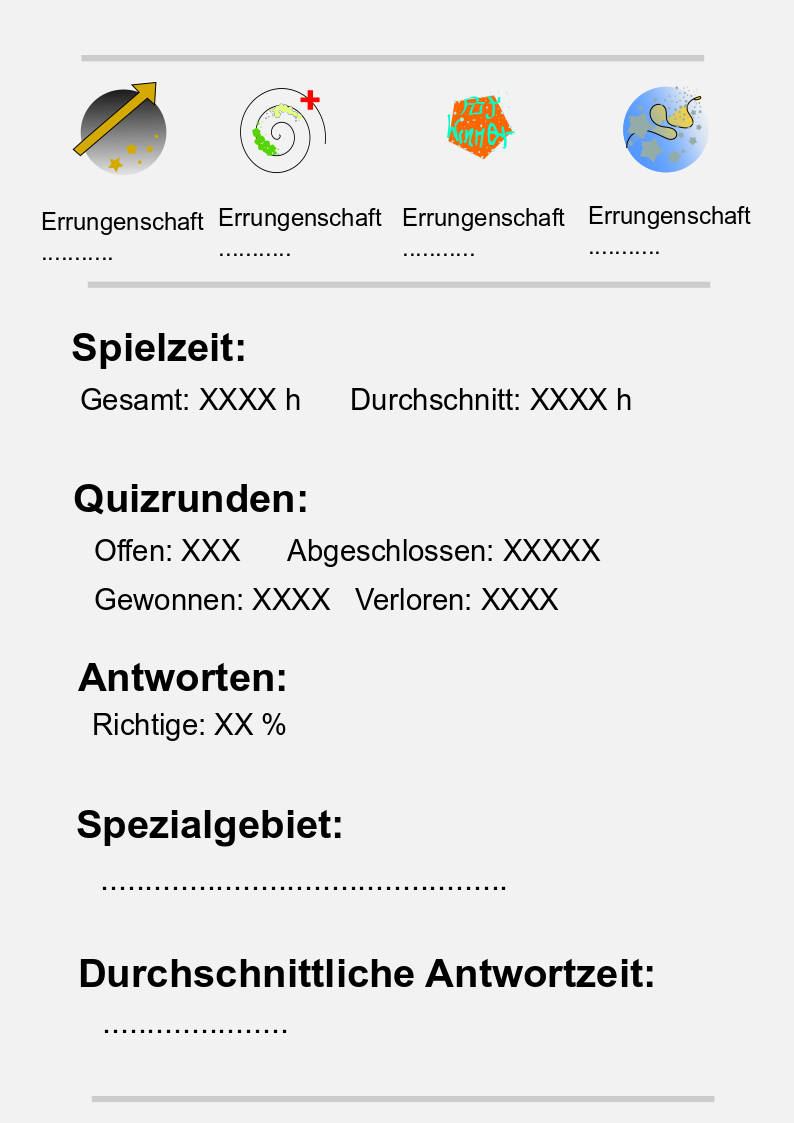
\includegraphics[height = 0.4\textheight]{Dashboard.png}
	\caption{Dashboardansicht für den User}
	\label{img:Dashboard}
\end{figure}

\begin{figure}
	\centering
	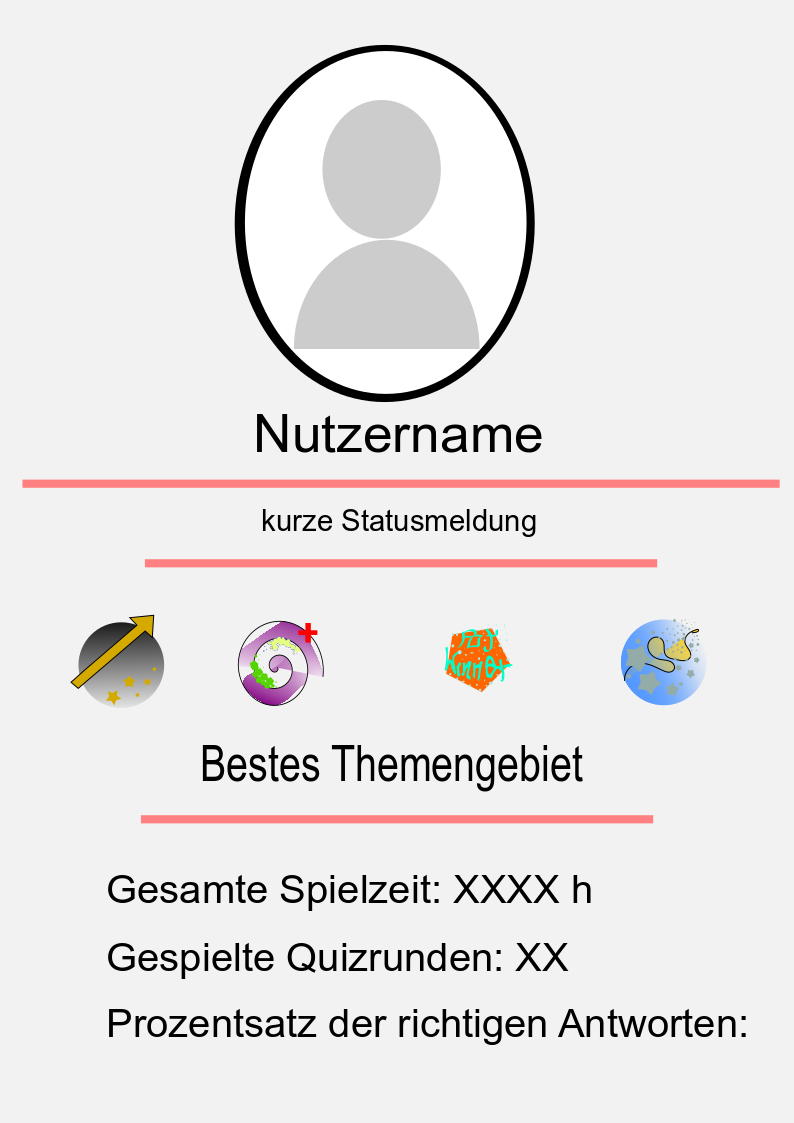
\includegraphics[height = 0.4\textheight]{Profil.png}
	\caption{Profilansicht für den User}
	\label{img:Profil}
\end{figure}

\begin{figure}
	\centering
	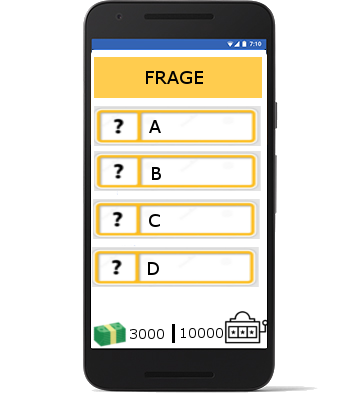
\includegraphics[height = 0.4\textheight]{version_2.png}
	\caption{Fragenansicht für den User}
	\label{img:Frage}
\end{figure}


\Chapter{Grundsätzliche Struktur - und Entwurfsprinzipien}
Die gewählte Architektur ist eine Server-Client-Architektur. Sie ist unter Abbildung \ref{img:Architektur} schematisch dargestellt. Die erste Schicht bildet die PostgreSQL Datenbank inkl. Datenbankserver. Die Middleware besteht aus einem Server, welcher die Spiellogik händelt und einer REST-Schnittstelle. Der Client, also die eigentliche App und die Administrationsoberfläche, kommuniziert ausschließlich über REST mit Server und Datenbank. Der Server hingegen kann über ein objektrelationales Datenbankmapping mittels Hibernate direkt auf die Datenbank zugreifen. Dazu werden spezielle Klassen (DataAccessObjects, DAO) verwendet.

\begin{figure}
	\centering
	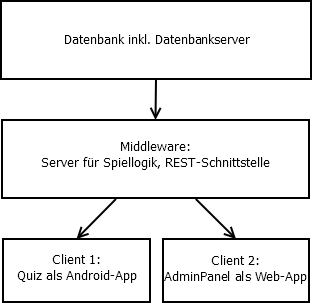
\includegraphics[height = 0.4\textheight]{Architektur.png}
	\caption{Architektur der Anwendung}
	\label{img:Architektur}
\end{figure}


\Chapter{Struktur - und Entwurfsprinzipien einzelner Pakete}


\Chapter{Datenmodell}


\Chapter{Glossar}

\end{document}